\documentclass[12pt]{article}
\usepackage[breaklinks=true]{hyperref}
\usepackage[margin=0.75in]{geometry}

\usepackage{graphicx}
\usepackage{color}

\definecolor{pblue}{rgb}{0.13,0.13,1}
\definecolor{pgreen}{rgb}{0,0.5,0}
\definecolor{pred}{rgb}{0.9,0,0}
\definecolor{pgrey}{rgb}{0.46,0.45,0.48}

\usepackage{listings}
\lstset{language=Java,
  showspaces=false,
  showtabs=false,
  tabsize=2,
  breaklines=true,
  showstringspaces=false,
  breakatwhitespace=true,
  commentstyle=\color{pgreen},
  keywordstyle=\color{pblue},
  stringstyle=\color{pred},
  basicstyle=\ttfamily,
  frame=single,
  moredelim=[il][\textcolor{pgrey}]{$$},
  moredelim=[is][\textcolor{pgrey}]{\%\%}{\%\%}
}

\title{Concurrency: Writing Multithreaded Programs in Java}
\author{
	Melvyn Ian Drag
}
\date{\today}


\begin{document}
\maketitle

\begin{abstract}
Up until now we've written \textbf{serial} code. Today we will learn to write
\textbf{concurrent} code. In other words, before we only programmed our machines
to do one thing at a time. Now we will write programs that multitask - or at
least give the illusion of multitasking.
\end{abstract}

\section{}


\begin{figure}[h]
  \centering
    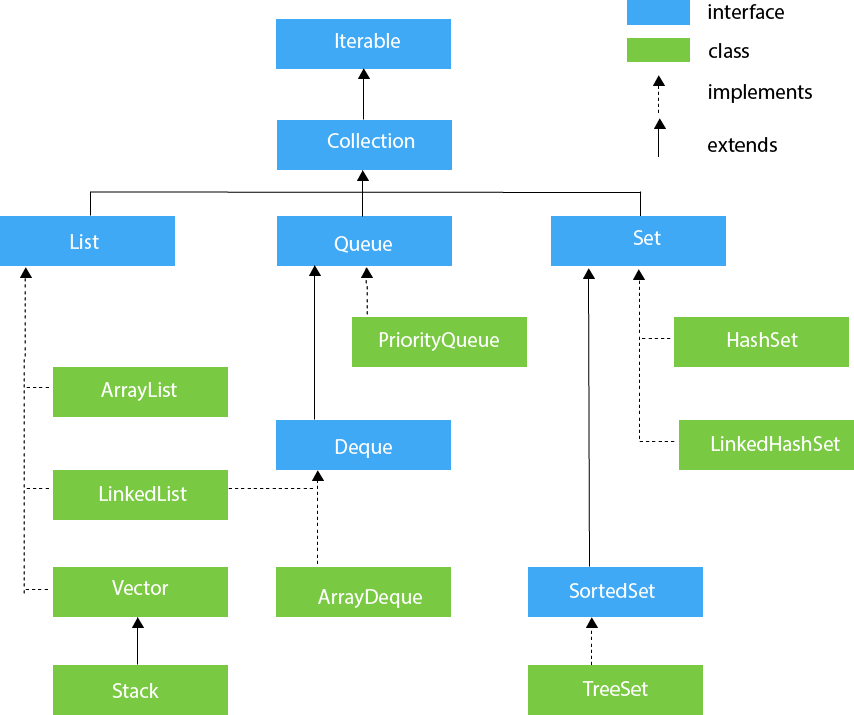
\includegraphics[width=0.5\textwidth]{java-collection-hierarchy.png}
  \caption{Illustration of a variety of classes which implement the Collection class.}
\end{figure}

\end{document}
